% FADO --- CISUC template, Beamer version.
% Compiles with pdfLaTeX, XeLaTeX, or LuaLaTeX (run twice for the TikZ overlays).
\documentclass[aspectratio=169]{beamer}
\usepackage{geometry}
\geometry{paperwidth=13.333in,paperheight=7.5in}
\usepackage{iftex}
\usepackage{tikz}
\usetikzlibrary{arrows.meta}
\usepackage{booktabs}
\usepackage{multirow}
\usepackage{amsmath}
\usepackage{array}

% ---- fonts (engine-agnostic; TeXLive-bundled Helvetica/Courier clones, no fontspec) ----
\ifPDFTeX\usepackage[utf8]{inputenc}\fi
\usepackage[T1]{fontenc}
\usepackage{textcomp}
\usepackage{tgheros}   % Helvetica clone (Arial-like) sans
\usepackage{tgcursor}  % Courier clone mono
\renewcommand{\familydefault}{\sfdefault}
\newcommand{\monofont}{\ttfamily}

% ---- colours ----
\definecolor{cred}{HTML}{DA0725}
\definecolor{ink}{HTML}{141414}
\definecolor{body}{HTML}{262626}
\definecolor{grey}{HTML}{9A9A9A}
\definecolor{lgrey}{HTML}{C4C4C4}
\definecolor{rulec}{HTML}{2A2A2A}
\definecolor{green}{HTML}{2E9E5B}
\definecolor{amber}{HTML}{C77A18}

\setbeamercolor{normal text}{fg=body}
\setbeamercolor{itemize item}{fg=cred}
\setbeamercolor{itemize subitem}{fg=cred}
\setbeamercolor{itemize subsubitem}{fg=cred}
\setbeamercolor{enumerate item}{fg=cred}
\setbeamercolor{enumerate subitem}{fg=cred}
\setbeamercolor{enumerate subsubitem}{fg=cred}
\setbeamercolor{item projected}{fg=cred}
\setbeamertemplate{navigation symbols}{}
\setbeamersize{text margin left=0pt,text margin right=0pt}

% ---- running header (shown on non-plain frames) ----
\newcommand{\hdrsec}{}
\newcommand{\hdrpg}{}
\newcommand{\pageset}[2]{\renewcommand{\hdrsec}{#1}\renewcommand{\hdrpg}{#2}}
\setbeamertemplate{headline}{%
  \vskip3mm%
  \makebox[\paperwidth][c]{%
    \hspace{9mm}%
    \parbox[t]{4.2in}{\monofont\color{grey}\fontsize{9}{11}\selectfont
      FADO: A Reaction Controller for Fairness-\\ Aware Online Learning Under Concept Drift}%
    \hfill
    \parbox[t]{4.2in}{\centering\monofont\color{grey}\fontsize{10}{12}\selectfont \hdrsec}%
    \hfill
    \parbox[t]{2.6in}{\raggedleft\monofont\fontsize{13}{15}\selectfont
      \textbf{\color{ink}\hdrpg}{\color{grey}/21}}%
    \hspace{9mm}%
  }%
}
\setbeamertemplate{footline}{}
\setbeamertemplate{frametitle}{}

% ---- helpers (absolute placement via TikZ overlay) ----
% \tb{width-in}{x-in}{y-in}{content}  --- anchored top-left at (x,y) from page NW
% optional #1 = extra node options (use font=... for large text so spacing scales)
\newcommand{\tb}[5][]{\begin{tikzpicture}[remember picture,overlay]%
  \node[anchor=north west,inner sep=0pt,outer sep=0pt,text width=#2in,align=left,#1]
    at ([xshift=#3in,yshift=-#4in]current page.north west){\raggedright #5\par};\end{tikzpicture}}
\newcommand{\fs}[2]{\fontsize{#1}{#2}\selectfont}
\newcommand{\hrl}[3]{\tb{#3}{#1}{#2}{{\color{lgrey}\rule{#3in}{0.9pt}}}}
% square outline cell with centred label: \boxcell{x}{y}{size-in}{label}
\newcommand{\boxcell}[4]{\begin{tikzpicture}[remember picture,overlay]%
  \node[draw=lgrey,line width=0.8pt,anchor=north west,minimum width=#3in,minimum height=#3in,
    align=center,text=ink,font=\fontsize{14}{16}\selectfont]
    at ([xshift=#1in,yshift=-#2in]current page.north west){#4};\end{tikzpicture}}
% arrow from (x1,y1) to (x2,y2) in inches from page NW
\newcommand{\parrow}[4]{\begin{tikzpicture}[remember picture,overlay]%
  \draw[-{Latex[length=2mm]},line width=1.3pt,ink]
    ([xshift=#1in,yshift=-#2in]current page.north west)--([xshift=#3in,yshift=-#4in]current page.north west);\end{tikzpicture}}
% column helpers (fixed y per slide type) --- defined once, avoid in-frame defs
\newcommand{\colblk}[4]{%
  \tb{3.5}{#1}{2.45}{\bfseries\color{ink}\fs{17}{20}#2}%
  \tb{3.5}{#1}{2.9}{\itshape\color{grey}\fs{12}{14}#3}%
  \hrl{#1}{3.32}{3.3}%
  \tb{3.3}{#1}{3.5}{\color{body}\fs{13.5}{17}#4}}
\newcommand{\phaseblk}[4]{%
  \tb{3.5}{#1}{2.5}{\bfseries\color{cred}\fs{17}{20}#2}%
  \tb{3.5}{#1}{2.95}{\itshape\color{grey}\fs{13}{15}#3}%
  \hrl{#1}{3.35}{3.1}%
  \tb{3.2}{#1}{3.5}{\color{body}\fs{13}{16}#4}}
\newcommand{\dcolblk}[3]{%
  \tb{3.6}{#1}{2.55}{\bfseries\color{ink}\fs{16}{19}#2}%
  \hrl{#1}{3.35}{3.3}%
  \tb{3.4}{#1}{3.5}{\color{body}\fs{14}{18}#3}}
\newcommand{\ctitle}[1]{\tb[font=\fontsize{28}{28}\selectfont\bfseries]{11.6}{0.85}{1.4}{\color{ink}#1}}
\newcommand{\divider}[2]{\tb[font=\fontsize{40}{46}\selectfont\bfseries]{11.3}{1.0}{3.05}{%
  \centering{\color{cred}#1.\ }{\color{ink}#2}}}
\newcommand{\body}[1]{\tb{7.1}{0.85}{2.5}{\color{body}\fs{17}{23}\setlength{\parskip}{9pt}#1}}
\newcommand{\centerimage}[3]{%
  \pgfmathsetmacro{\centerimagex}{(13.333-#1)/2}%
  \tb{#1}{\centerimagex}{#2}{\includegraphics[width=#1in]{#3}}}
\newcommand{\codepanel}[3]{%
  \tb{5.45}{#1}{2.25}{\bfseries\color{cred}\fs{16}{19}#2}%
  \hrl{#1}{2.8}{5.45}%
  \tb{5.45}{#1}{3.05}{\color{body}\ttfamily\fs{10.2}{12.5}#3}}
\newcommand{\slidefoot}[1]{%
  \tb{11.6}{0.85}{6.45}{\centering\color{grey}\fs{13}{16}#1}}
\newcommand{\question}[4]{\hrl{8.35}{#1}{4.1}\tb{4.1}{8.35}{#2}{\fs{14}{18}{\color{cred}\bfseries #3}\par\smallskip{\color{ink}#4}}}
\newcommand{\outlineitem}[2]{\color{cred}\bfseries #1.\hspace{0.6em}{\color{ink}#2}\par}
\newcommand{\titleSlide}[2]{%
  \tb[font=\fontsize{46}{50}\selectfont\bfseries]{11.4}{0.9}{2.4}{\color{ink}#1}%
  \tb[font=\fontsize{30}{36}\selectfont\bfseries]{11.4}{0.9}{3.4}{\color{ink}#2}%
  \tb{2.5}{0.9}{6.75}{
\includegraphics[width=2.5in]{assets/cisuc_logo.png}}}

\begin{document}

% ===================================================== 1 LOGO
\begin{frame}[plain]
  \tb{4.6}{4.37}{3.35}{
\includegraphics[width=4.6in]{assets/cisuc_logo.png}}
\end{frame}

% ===================================================== 2 TITLE
\begin{frame}[plain]
  \titleSlide{FADO} {Meating 1}
  \tb{11}{0.92}{4.55}{\color{ink}\fs{19}{22}Tiago Silva}
  \tb{11}{0.92}{5.35}{\color{ink}\fs{14}{18}\textbf{CISUC \textperiodcentered{} Data-Centric AI Lab}\\
    {\color{body}\fs{14}{18}Department of Informatics Engineering, University of Coimbra}}
  \tb{2.5}{0.9}{6.75}{
\includegraphics[width=2.5in]{assets/cisuc_logo.png}}
\end{frame}

% ===================================================== 3 OUTLINE (01)
\pageset{Outline}{01}
\begin{frame}
  \ctitle{Outline}
  \begin{quote}
    \body{
      \begin{enumerate}
        \item \textbf{Overall Assessment};
        \item \textbf{The Depth Problem};
      \end{enumerate}
    }
  \end{quote}
\end{frame}

% ===================================================== S1 divider (02)
\pageset{First Submission's Assessment}{02}
\begin{frame}
  \ctitle{Overall Assessment}
  \body{
    \textbf{Strengths:}
    \begin{itemize}
      \item Significant problem, well written/organized;
      \item Improves fairness metrics maintaining predictive performance;
      \item Rigorous statistical evaluation, reproducible code.
    \end{itemize}
    \medskip
    \textbf{Weaknesses:}
      \begin{itemize}
        \item Doubts about novelty - Lack of Differentiation from prior work;
        \item Limited Theoretical Justification of parameters (Lack of Ablation Studies);
        \item Should Ablate the effect of each component of the proposed method;
        \item More datasets.
      \end{itemize}
  } 
\end{frame}

\pageset{Tree Depth}{03}
\begin{frame}
  \ctitle{Testing deeper trees with {\color{cred}\textit{\underline{limited}}} horsepower}
  \centerimage{5.5}{2}{assets/mask_updates.png}
  \body{
    \textbf{To ablate tree depth we must be faster \color{cred}\textit{\underline{faster}}!}
  }
  \slidefoot{A prediction is the sum of the products of the node decisions along the path to each leaf.}
\end{frame}

\pageset{Tree Depth}{04}
\begin{frame}
  \ctitle{Tree depth: mask products vs. recursive propagation}
  \codepanel{0.85}{Before: mask approach}{%
    logits $\leftarrow$ (inputs $\times$ weight $+$ bias) / temperature\\
    node\_decisions $\leftarrow$ activation(logits)\\[2pt]
    y $\leftarrow$ expand\_dims(node\_decisions)\\
    y\_repeated $\leftarrow$ repeat(y, num\_leaves)\\
    z $\leftarrow$ y\_repeated $\odot$ mask\\
    probs $\leftarrow$ relu(z) $+$ (ones $-$ relu($-$z)) $+$ mask $+$ $\epsilon$\\[2pt]
    for each leaf $\ell$:\\
    \hspace*{1em}leaf\_probs[$\ell$] $\leftarrow$ product(probs[:, :, $\ell$])\\
    \hspace*{1em}{\color{grey}\rmfamily\itshape\# materialise every node--leaf pair}\\[-1pt]
    \hspace*{1em}{\color{grey}\rmfamily\itshape\# repeat the product for every leaf}\\[2pt]
    prediction $\leftarrow$ leaf\_probs $\times$ $\theta$
  }
  \codepanel{7.0}{After: recursive updater}{%
    logits $\leftarrow$ (inputs $\times$ weight $+$ bias) / temperature\\
    node\_decisions $\leftarrow$ activation(logits)\\[2pt]
    root\_prob $\leftarrow$ 1\\
    leaf\_probs $\leftarrow$ traverse(root, root\_prob,\\
    \hspace*{1em}node\_decisions, depth)\\
    \hspace*{1em}{\color{grey}\rmfamily\itshape\# propagate only to valid child branches}\\[-1pt]
    \hspace*{1em}{\color{grey}\rmfamily\itshape\# reuse each partial path probability}\\[2pt]
    \hspace*{1em}prediction $\leftarrow$ leaf\_probs $\times$ $\theta$
  }
  \slidefoot{\textbf{Complexity goes from \color{cred}$O(B\times4^n)$ to $O(B\times2^n)$\color{grey}, where $n$ is the tree depth.}}
\end{frame}

\pageset{Tree Depth}{05}
\begin{frame}
  \ctitle{Tree depth: mask products vs. recursive \color{cred}\textit{\underline{performance}}}
  \tb{6.2}{0.85}{2.0}{
    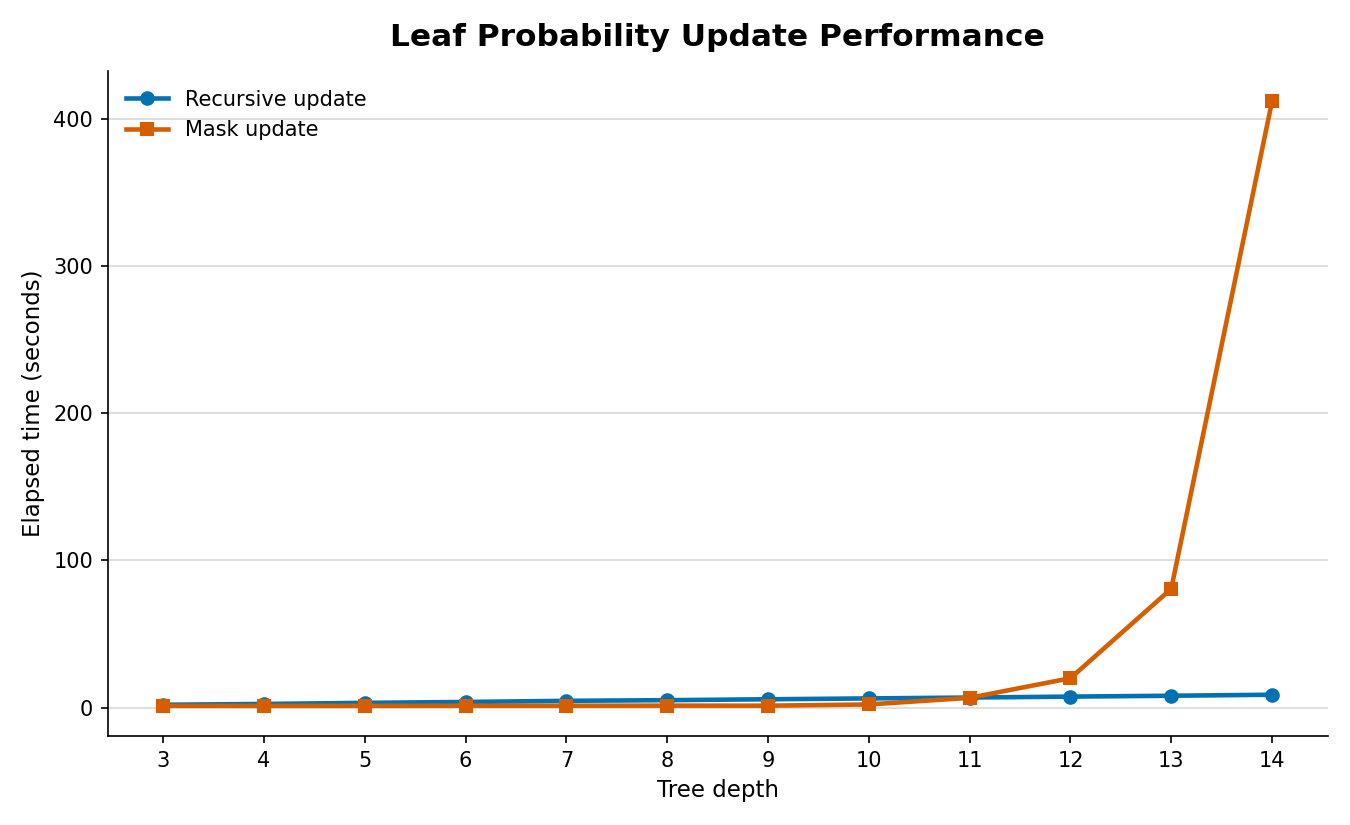
\includegraphics[width=6.2in]{assets/probability_updater_performance.png}
  }
  \tb{6.2}{7.0}{2.0}{
    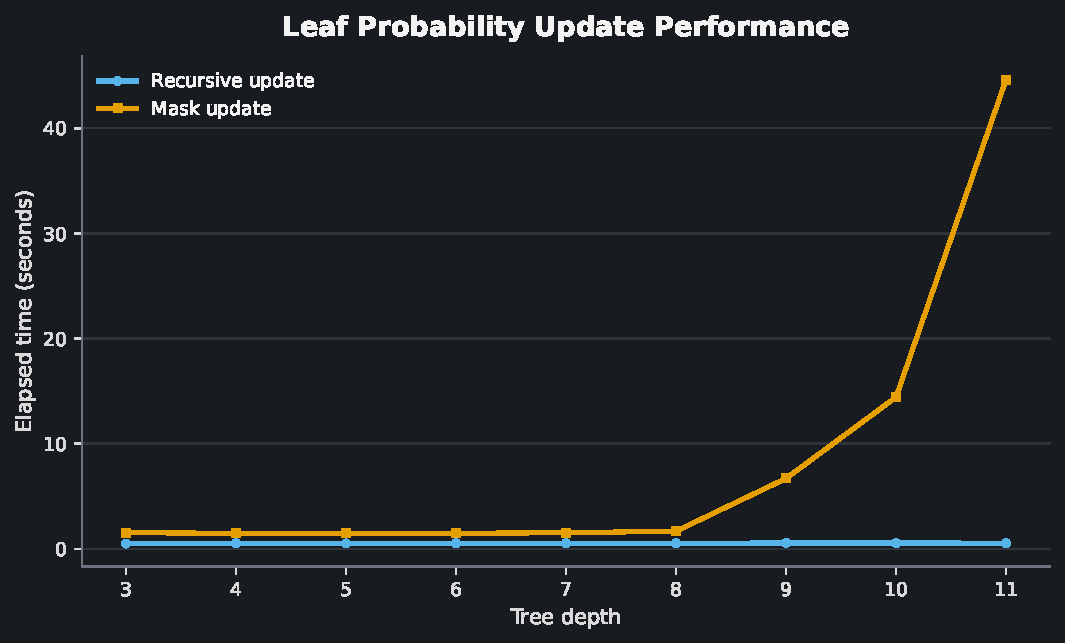
\includegraphics[width=6.2in]{assets/leaf_probability_update_performance.pdf}
  }
  \slidefoot{We can now ablate how trees' depth affect the forest's predictive and fairness metrics}
  \footnote{Stopped at n = 14 for GPU and n = 11 for CPU because the mask's runtime became unbearable.}

\end{frame}

\pageset{Online Fairness Metrics}{06}
\begin{frame}
  \ctitle{Rolling fairness metrics: incremental counters}
  \dcolblk{0.85}{Legacy recomputation}{
    Each sample rescans the complete fairness window for DP and EO.\\[5pt]
    Complexity: \color{cred}$O(NW)$\color{body}, where $W$ is the window size.
  }
  \dcolblk{4.85}{Incremental window}{
    Add the arriving sample and remove the expired sample from group counters.\\[5pt]
    Complexity: \color{green}$O(NA)$\color{body}, where $A$ is the number of groups.
  }
  \dcolblk{8.85}{Benchmark}{
    50,000 samples; window size 1,000; binary protected attribute.\\[5pt]
    \textbf{15.39$\times$ faster} with identical DP and EO at every timestep.
  }
  \slidefoot{The counter-based window preserves the metric values while avoiding repeated scans of the same samples.}
\end{frame}

\pageset{Current model performance}{07}
\begin{frame}
  \ctitle{Real \color{cred}\textit{\underline{impact}} \color{black}on model's \color{cred}\textit{\underline{performance}}}
  \body{
    For an adult dataset run (~32k samples) we were able to reduce from 37.12 minutes to \textit{\underline{13.22 minutes}}.
  }
  \slidefoot{We can now proceed to ablate tree depth!}
\end{frame}


\end{document}
